\documentclass[11pt]{article}

\usepackage[margin=1.5in]{geometry}

\usepackage{fancyhdr}
\pagestyle{fancy}
\newcommand\course{CSC 425}
\newcommand\hwnumber{1}
\newcommand\duedate{October 1, 2020}

\lhead{Oliver Tonnesen\\V00885732}
\chead{\textbf{\Large Assignment \hwnumber}}
\rhead{\course\\\duedate}


\usepackage{tikz}


\usepackage{amsmath, amssymb, mathtools}

\DeclarePairedDelimiter\abs{\lvert}{\rvert}%
\makeatletter
\let\oldabs\abs
\def\abs{\@ifstar{\oldabs}{\oldabs*}}

\usepackage{algorithm}
\usepackage[noend]{algpseudocode}

\begin{document}
\renewcommand{\thesubsection}{\thesection.\roman{subsection}}
\section{} % Section 1
Yes, a student can benefit by lying about their preferences.
We provide an example of this:

Given students $s_1$, $s_2$, and $s_3$, and hospitals $h_1$, $h_2$, and $h_3$ with preference lists as follows:
\begin{align*}
	s_1: h_2, h_1, h_3 &\qquad\qquad h_1: s_1, s_2, s_3 \\
	s_2: h_1, h_2, h_3 &\qquad\qquad h_2: s_2, s_1, s_3 \\
	s_3: h_1, h_2, h_3 &\qquad\qquad h_3: s_1, s_2, s_3
\end{align*}
the Gale-Shapley algorithm returns the following matching:
\newline
\newline
\begin{figure}[h]
\centering
\begin{tikzpicture}[black/.style={circle,draw,fill=black,inner sep=0pt, minimum width=4pt}]
\node at (1,2) (1) {$s_1$};
\node at (1,1) (2) {$s_2$};
\node at (1,0) (3) {$s_3$};
\node at (4,2) (A) {$h_1$};
\node at (4,1) (B) {$h_2$};
\node at (4,0) (C) {$h_3$};
\draw (1) -- (A);
\draw (2) -- (B);
\draw (3) -- (C);
\end{tikzpicture}
\end{figure}
\newline
But if student $s_1$ were to lie and submit the dishonest preference list $h_2,h_3,h_1$, the Gale-Shapley algorithm would return the following matching:
\newline
\newline
\begin{figure}[h]
\centering
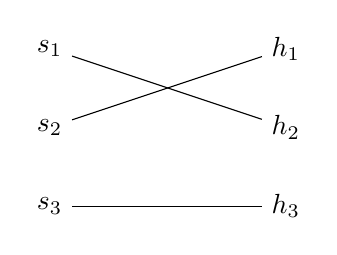
\begin{tikzpicture}[black/.style={circle,draw,fill=black,inner sep=0pt, minimum width=4pt}]
\node at (1,2) (1) {$s_1$};
\node at (1,1) (2) {$s_2$};
\node at (1,0) (3) {$s_3$};
\node at (4,2) (A) {$h_1$};
\node at (4,1) (B) {$h_2$};
\node at (4,0) (C) {$h_3$};
\draw (1) -- (B);
\draw (2) -- (A);
\draw (3) -- (C);
\end{tikzpicture}
\end{figure}
\newline
Notice that $s_1$ was matched with a hospital higher on their actual preference list this time than they were originally.


\section{} % Section 2
\subsection{} % Section 2.i
Instability in this case includes both the preferences of the students and the hospitals, and also the number of positions available at a hospital.
That is, a student--hospital pair $s$--$h$ can be unstable if either of the following are true:
\begin{enumerate}
	\item $s$ prefers $h$ to the hospital it's matched with, and $h$ prefers $s$ to a student it's matched with.
	\item $h$ prefers $s$ to a student it's matched with, and $s$ is not matched to any hospital.
\end{enumerate}


\subsection{} % Section 2.ii
The main idea of our new algorithm is to compare a prospective student to a hospital's least-preferred student wherever we would normally compare it to the hospital's matched student.

The object our new algorithm produces is not guaranteed to be a matching since hospitals are no longer restricted to a single student, so instead we return a graph.

\begin{algorithm}
\begin{algorithmic}
\Function{Modified-Gale-Shapley}{\emph{preference lists for hospitals and students}}
\State Initialize $M$ to empty graph.
\While{some hospital $h$ has an open spot and hasn't offered a position to every student}
	\State $s$ $\gets$ first student on $h$'s list to whom $h$ has not yet offered a position.
	\If{$s$ is unmatched}
		\State Add $h$--$s$ to $M$.
	\ElsIf{$s$ prefers $h$ to current hospital $h'$}
		\State Replace $h'$--$s$ with $h$--$s$ in $M$.
	\Else
		\State $s$ rejects $h$.
	\EndIf
\EndWhile
\State \Return $M$
\EndFunction
\end{algorithmic}
\end{algorithm}


We claim that the above algorithm produces a stable graph, with ``stability'' is defined as above.

Let $M$ be the graph returned by the algorithm, and suppose for the sake of contradiction that there exists a student $s$ and a hospital $h$ such that $h$ prefers $s$ to its least-preferred matched student, and $s$ prefers $h$ to its matched hospital or is unmatched.

\noindent
\underline{Case 1} (s is matched):
\newline

\indent
\underline{Case 1.1} ($h$ never proposed to $s$): Hospitals propose in descending order of preference, so it prefers $s'$ to $s$, a contradiction.
\newline

\indent
\underline{Case 1.2} ($h$ proposed to $s$): Once a student is matched to a hospital, it only becomes unmatched if it is offered a position at a more preferred hospital, so it must be the case that $s$ prefers its currently-matched hospital to $h$, a contradiction.
\newline

\underline{Case 2} ($s$ is unmatched): $h$ prefers $s$ to its currently matched student, so it must have offered a position to $s$ before it offered a position to $s'$, so $s$ must be matched, a contradiction.

Thus $M$ has no unstable pair $s$--$h$, as desired.


\section{} % Section 3
Given a schedule, we define an \textbf{\underline{inversion}} to be a pair of jobs $i$, $j$ that, when swapped, incur a lesser penalty than before they were swapped; in other words:
\[f_iw_i + f_jw_j > (f_j-t_i)w_j + f_jw_i\]

We can manipulate the above inequality to obtain an equivalent one:
\[\frac{t_i}{w_i} > \frac{t_j}{w_j}\]

An \textbf{\underline{adjacent inversion}} is an inversion in which $i$ and $j$ come one after the other in a given schedule.
We claim that if a schedule has an inversion, then it has an adjacent inversion.

Let $i$--$j$ be a closest inversion (with $i$ coming before $j$), and let $k$ be the job to the right of $i$.
Suppose for a contradiction that $i$ and $k$ are not inverted, so $\frac{t_i}{w_i} \le \frac{t_k}{w_k}$.
But then $\frac{t_k}{w_k} \ge \frac{t_i}{w_i} > \frac{t_j}{w_j}$, so $k$--$j$ is a closer inversion -- a contradiction, so $i$ and $k$ are inverted.

We now claim an inversion-free schedule is optimal. Note that inversion-free schedules are unique up to same-weight, same-duration jobs.

Let $S$ be an optimal schedule with fewest inversions.
If it has no inversions, we're done.
Otherwise, $S$ has an inversion.
Remove it, and $S$ has no increased in total weight, but has fewer inversions, a contradiction.
Thus an optimal schedule indeed has no inversions.

It is now clear that we can use the greedy algorithm weighted by $\frac{t_i}{w_i}$ to obtain an inversion-free -- thus optimal -- schedule.


\section{} % Section 4
Begin by calculating the distance between each pair of points.
Denote each distance $d_{ij}$.
Note that this can be done in $\binom{n}{2}\in\Theta(n^2)$ operations.

Let $G$ be the complete graph with vertex set $U$ and let $M_G=(S_G,I_G)$ e the graphic matroid defined by $G$.
Define $w: S_g \rightarrow \mathbb{R}^+$ by $w(i,j) = K - d_{ij}$, where $K = \max_{i,j}\{d_{ij}\}$.

We now run the greedy algorithm on $(M,w)$ to obtain a maximal independent set, or in this case a spanning tree of $G$ with minimum ``weight'', where weight is $\sum_{i,j} d_{ij}$.
The last $k-1$ edges we added to the tree had the $k-1$ largest values of $w(i,j)$, and thus the smallest values of $d_{ij}$; furthermore, removing them will leave us with a forest of $k$ trees in $G$.
Thus the edge we removed with the largest value of $w(i,j)$ has the smallest value of $d_{ij}$.
If we now view the $k$ trees in the resulting forest as clusters of points on the plane, our forest represents a $k$-clustering, and this edge represents the minimum distance between any pair of points in different clusters -- or the spacing of our $k$-clustering.

Given $n$ points, this algorithm runs in time proportional to $n^2$, whereas a brute-force algorithm testing all $\binom{n-1}{k-1}$ of the possible $k$-clusterings would take time proportional to $n!$.


\section{} % Section 5
Recall the three properties defining a matroid:
\begin{enumerate}
\item $S$ is a finite set.
\item $I$ is a nonempty family of subsets of $S$ such that if $B \in I$ and $a \subseteq B$, then $A \in I$.
\item If $A,B \in I$ and $\abs{A} < \abs{B}$, then there exists $x \in B \setminus A$ such that $A \cup \{x\} \in I$.
\end{enumerate}

To show that that $(S,I)$ is a matroid, we show that it satisfies the above three properties:
\begin{enumerate}
\item Given.
\item Let $A \subseteq B \in I$, and let $i \in \{1,2,\ldots,k\}$.
$A \subseteq B$, so $\abs{A \cap S_i} \le \abs{B \cap S_i} \le 1$, so $A \in I$.
\item Let $A,B \in I$ such that $\abs{A} < \abs{B}$.
$B$ can contain no more than $k$ elements since $S_1,\ldots,S_k$ are disjoint, so $A$ can contain no more than $k-1$ elements.
This means there is at least one set $S_i$ for which $\abs{B \cap S_i} = 1$ and $\abs{A \cap S_i} = 0$.
Thus let $x \in B \cap S_i$, then $\abs{\left(A \cup \{x\}\right) \cap S_i} = \abs{\{x\}} = 1$, and so $A \cup \{x\} \in I$, as desired.
\end{enumerate}


\end{document}
